\documentclass{beamer}
\usepackage[utf8]{inputenc}

\usetheme{Madrid}
\usecolortheme{default}
\usepackage{txfonts}
\usepackage{listings}
\usepackage{adjustbox}
\usepackage{tabularx}
\usepackage{lmodern}
\usepackage{circuitikz}
\usepackage{tikz}

\usepackage{gvv}
\usepackage{cite}
\usepackage{amsmath,amssymb,amsfonts,amsthm}
\usepackage{algorithmic}
\usepackage{graphicx}
\usepackage{textcomp}
\usepackage{xcolor}
\usepackage{txfonts}
\usepackage{listings}
\usepackage{enumitem}
\usepackage{mathtools}
\usepackage{gensymb}
\usepackage{comment}
\usepackage{tkz-euclide} 
\usepackage{listings}                                      
\def\inputGnumericTable{}                                
\usepackage{color}                                            
\usepackage{array}                                            
\usepackage{longtable}
\usepackage{multicol}
\usepackage{calc}                                             
\usepackage{multirow}                                         
\usepackage{hhline}                                           
\usepackage{ifthen}

\setbeamertemplate{page number in head/foot}[totalframenumber]

\usepackage{tcolorbox}
\tcbuselibrary{minted,breakable,xparse,skins}



\definecolor{bg}{gray}{0.95}
\DeclareTCBListing{mintedbox}{O{}m!O{}}{%
  breakable=true,
  listing engine=minted,
  listing only,
  minted language=#2,
  minted style=default,
  minted options={%
    linenos,
    gobble=0,
    breaklines=true,
    breakafter=,,
    fontsize=\small,
    numbersep=8pt,
    #1},
  boxsep=0pt,
  left skip=0pt,
  right skip=0pt,
  left=25pt,
  right=0pt,
  top=3pt,
  bottom=3pt,
  arc=5pt,
  leftrule=0pt,
  rightrule=0pt,
  bottomrule=2pt,
  toprule=2pt,
  colback=bg,
  colframe=orange!70,
  enhanced,
  overlay={
    \begin{tcbclipinterior}
    \fill[orange!20!white] (frame.south west) rectangle ([xshift=20pt]frame.north west);
    \end{tcbclipinterior}},
  #3,
}
\lstset{
    language=python,
    basicstyle=\ttfamily\small,
    keywordstyle=\color{blue},
    stringstyle=\color{orange},
    commentstyle=\color{green!60!black},
    numbers=left,
    numberstyle=\tiny\color{gray},
    breaklines=true,
    showstringspaces=false,
}

% --- Define SPICE Language ---
\lstdefinelanguage{Spice}{
    morekeywords={.tran, .dc, .ac, .model, .subckt, .ends, .include, .lib, .param, .options, .print, .plot, .end, .ic},
    morecomment=[l]{*}, % SPICE comments start with an asterisk
    morestring=[b]",
    sensitive=false,
}

% --- Define SPICE Style ---
\lstdefinestyle{spice}{
    language=Spice,
    basicstyle=\ttfamily\small,
    keywordstyle=\color{blue}\bfseries,
    stringstyle=\color{red},
    commentstyle=\color{green!60!black}\itshape,
    numbers=left,
    numberstyle=\tiny\color{gray},
    breaklines=true,
    showstringspaces=false,
    frame=single, % Adds a subtle border around the code
    rulecolor=\color{gray!40},
    backgroundcolor=\color{gray!5},
}

\title 
{1.1.31}
\date{}


\author 
{Sai Sreevallabh - EE25BTECH11031}



\begin{document}

\frame{\titlepage}

\begin{frame}{Question}

 The probes of a non-isolated, two-channel oscilloscope are clipped to points A, B and C in the circuit as shown. $V_{\text{in}}$ is a square wave of a suitable low frequency. 
The display on Ch$_1$ and Ch$_2$ are as shown on the right. Then the Signal and Ground probes $S_1, G_1$ and $S_2, G_2$ of Ch$_1$ and Ch$_2$ respectively are connected to points

    
\end{frame}

\begin{frame}{Figure}

\begin{figure}
    \centering
    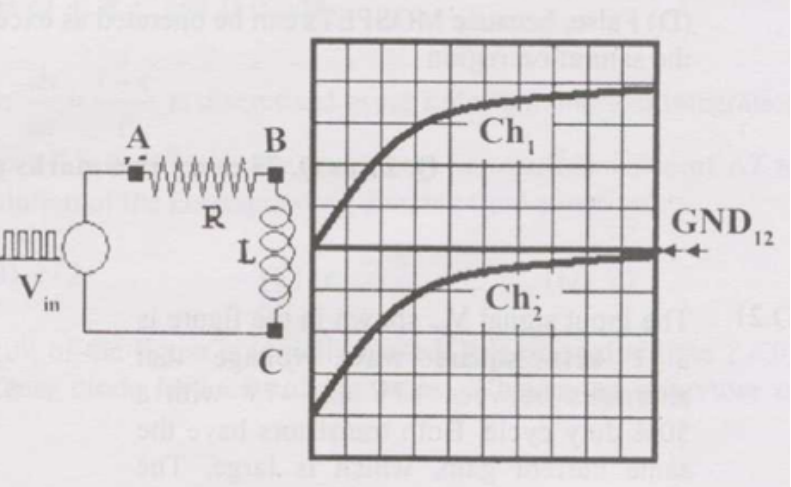
\includegraphics[width=0.75\linewidth]{Figs/question.png}
\end{figure}
    
\end{frame}

\begin{frame}{Options}

\begin{itemize}
    \item a) A,B,C,A
    \item b) A,B,C,B
    \item c) C,B,A,B
    \item d) B,A,B,C
\end{itemize}

\end{frame}

\begin{frame}{Theoretical Solution}

The DSO plots voltage vs time graphs of the signal with respect to the chosen ground, as per the clipping of the probes. \\

A non-isolated oscilloscope has the ground pins of both the channel permanently connected to each other and they are also connected to the Earth ground of the wall outlet. If the ground probes are not connected to the same node, then the output will be flawed. 

For the RL Circuit given in the figure, let the current be $i$. The circuit is described by the equation

\begin{align*}
V_{in} &= iR + L\frac{di}{dt}\\
\end{align*}


\end{frame}

\begin{frame}{Theoretical Solution:}

In s-domain, the inductor is modelled as a resistor with a resistance $sL$. Hence, the above given circuit is a voltage divider circuit with the transfer function of the voltage across the resistor given as :
\begin{align}
    H(s) = \frac{V_R(s)}{V_{in}(s)} = \frac{R}{sL + R} =  \frac{R/L}{s + R/L}
\end{align}

Hence, we have
\begin{align}
    V_R(s) = \frac{R/L}{s + R/L}V_{in}(s)\\
    \implies V_R(s) = \frac{V_{in}(R/L)}{s\brak{s + R/L}}
\end{align}


    
\end{frame}

\begin{frame}{Theoretical Solution:}

Breaking the equation into simpler fractions:
\begin{align}
    V_R(s) &= \frac{V_{in}}{s} - \frac{V_{in}}{s + R/L}
\end{align}

Using the below Inverse Laplace Transforms, we can convert back to time domain
\begin{align*}
    \mathcal{L}^{-1}\left\{\frac{1}{s}\right\} &= 1 \\
    \mathcal{L}^{-1}\left\{\frac{1}{s - a}\right\} &= e^{at} \implies \mathcal{L}^{-1}\left\{\frac{1}{s + R/L}\right\} = e^{-\frac{R}{L}t}
\end{align*}
The time domain solution:
\begin{align}
    \implies V_R\brak{t} &= V_{in}\brak{1 - e^{-\frac{R}{L}t}}
\end{align}
    
\end{frame}

\begin{frame}{Theoretical Solution}

The time domain solution:
\begin{align}
    \implies V_R\brak{t} &= V_{in}\brak{1 - e^{-\frac{R}{L}t}}
\end{align}

The waveform of Channel-1 of the DSO corresponds to this above equation. Hence, the signal probe ($S_1$) of the first channel is connected to point $A$ and ground probe ($G_1$) is connected to point $B$. 
    
\end{frame}



% \begin{frame}{Theoretical Solution:}

% Converting them to s-domain
% \begin{align*}
%     \mathcal{L}\{i(t)\} &= I(s) \\
%     \mathcal{L}\left\{\frac{di(t)}{dt}\right\} &= sI(s) - i(0) = sI(s) \\
%     \mathcal{L}\{V_0\} &= \frac{V_0}{s}
% \end{align*}

% The equation in s-domain is 
% \begin{align}
%     R I(s) + L[sI(s)] &= \frac{V_0}{s}\\
%     \implies  I(s) &= \frac{V_0/L}{s(s + R/L)}
% \end{align}
    
% \end{frame}

% \begin{frame}{Theoretical Solution:}

% Breaking the equation into simpler fractions:
% \begin{align}
%     I(s) &= \frac{V_0/R}{s} - \frac{V_0/R}{s + R/L}
% \end{align}

% Using the below Inverse Laplace Transforms, we can convert back to time domain
% \begin{align*}
%     \mathcal{L}^{-1}\left\{\frac{1}{s}\right\} &= 1 \\
%     \mathcal{L}^{-1}\left\{\frac{1}{s - a}\right\} &= e^{at} \implies \mathcal{L}^{-1}\left\{\frac{1}{s + R/L}\right\} = e^{-\frac{R}{L}t}
% \end{align*}

% \end{frame}

% \begin{frame}{Theoretical Solution}
% Applying the above Inverse Laplace Transforms, we get the below time-domain equation
% \begin{align}
%     i(t) &= \frac{V_0}{R} \left(1 - e^{-\frac{R}{L}t}\right)
% \end{align}
% Since, $V_R(t) = Ri(t)$
% \begin{align}
%     \implies V_R\brak{t} &= V_{in}\brak{1 - e^{-\frac{R}{L}t}}
% \end{align}

% The waveform of Channel-1 of the DSO corresponds to this above equation. Hence, the signal probe ($S_1$) of the first channel is connected to point $A$ and ground probe ($G_1$) is connected to point $B$. 
    
% \end{frame}

\begin{frame}{Theoretical Solution}
    Using $V_L = V_{in} - V_R$ we get
    \begin{align*}
        V_L = V_{in}e^{-\frac{R}{L}t}
    \end{align*}

This expression corresponds to the waveform which begins at $V_{in}$ at $t = 0$ and exponentially decays, with the X-axis as an asymptote. The waveform corresponding to Channel-2 is the negative of this exponentially decaying curve. \\
\noindent Hence, we can conclude that $S_2$ is connected to $C$ and $G_2$ is connected to $B$. 
This is consistent with the fact that the ground probes of both the channels should be connected to the same node. 
\vspace{0.3cm}

\boxed{Answer: B)\  A,B,C,B}
    
\end{frame}

\begin{frame}[fragile]
    \frametitle{Simulation Code (Python)}
    \begin{lstlisting}
import numpy as np
import sympy as sp
import matplotlib.pyplot as plt

Vin = 5.0
R = 1000.0
L = 0.01
T = L/R #Time constant

t_int = np.linspace(0, 5*T, 1000)

t = sp.symbols('t')
i = sp.Function('i')(t)
s = sp.symbols('s')

#Inputting the differential equation
de = sp.Eq(L*(sp.diff(i, t)) + R*i , Vin)

    \end{lstlisting}
 
    
\end{frame}

\begin{frame}[fragile]
    \frametitle{Simulation Code (Python)}
    \begin{lstlisting}
#Converting the equation to Laplace Transform
l_lhs = sp.laplace_transform(de.lhs, t, s, noconds = True)
l_rhs = sp.laplace_transform(de.rhs, t, s, noconds = True)

l_eq = sp.Eq(l_lhs, l_rhs)

#Initial Conditions for solving
initial_conditions = {i.subs(t, 0): 0}
l_eq_subbed = l_eq.subs(initial_conditions)

#Solving the s-domain equation
I_s = sp.laplace_transform(i, t, s, noconds=True)
I_s_solution = sp.solve(l_eq_subbed, I_s)[0]

#Getting the time-domain solution
i_t_sp = sp.inverse_laplace_transform(I_s_solution, s, t)

    \end{lstlisting}
 
    
\end{frame}

\begin{frame}[fragile]
    \frametitle{Simulation Code (Python)}
    \begin{lstlisting}
i_t = sp.lambdify(t, i_t_sp, modules=['numpy'])
i_vals = i_t(t_int)

Vr = R*i_vals
Vl = Vin - Vr

plt.plot(t_int, Vr, color = 'red', label = "Ch1")
plt.plot(t_int, -Vl, color = 'blue', label = "Ch2")
plt.axhline(y=5.0, color='gray', linestyle='--')


    \end{lstlisting}
 
    
\end{frame}

\begin{frame}[fragile]
    \frametitle{Simulation Code (Python)}
    \begin{lstlisting}
ax = plt.gca()
ax.spines['top'].set_color('none')
ax.spines['bottom'].set_position('zero')
ax.spines['right'].set_color('none')
ax.spines['left'].set_position('zero')
plt.legend(loc='best')

plt.minorticks_on()
plt.grid(which='major', linestyle='-', linewidth='0.6', color='gray')
plt.grid(which='minor', linestyle=':', linewidth='0.5', color='gray')


plt.savefig("../Figs/laplace.png")
plt.show()

    \end{lstlisting}
 
    
\end{frame}


\begin{frame}{Simulation Plot}

\begin{figure}
    \centering
    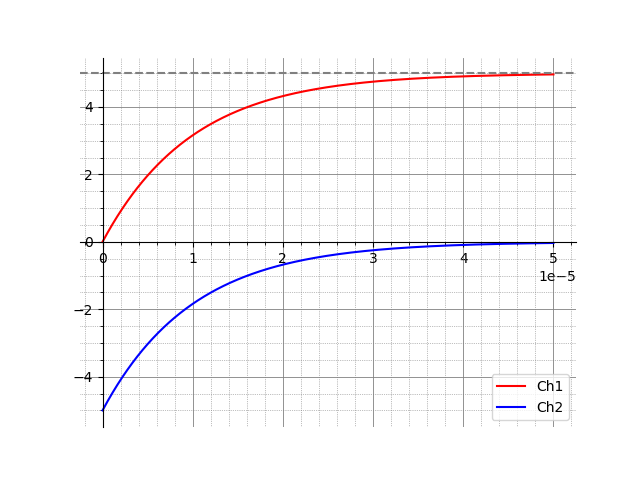
\includegraphics[width=0.9\linewidth]{Figs/laplace.png}
\end{figure}
    
\end{frame}

% \begin{frame}[fragile]
% \frametitle{Simulation Code (NGSPICE)}

% \begin{lstlisting}[style = spice]
% *1.1.31

% V1 in 0 PULSE(0 5 0 1ns 1ns 0.5s 1s)
% R1 in x 1k
% L1 x 0 10m

% .control
% tran 0.01us 50us

% let Ch1 = v(in) - v(x)
% let Ch2 = -v(x)

% plot Ch1 Ch2
% .endc


% \end{lstlisting}
    
% \end{frame}

% \begin{frame}{Simulation Plot NGSPICE}

% \begin{figure}
%     \centering
%     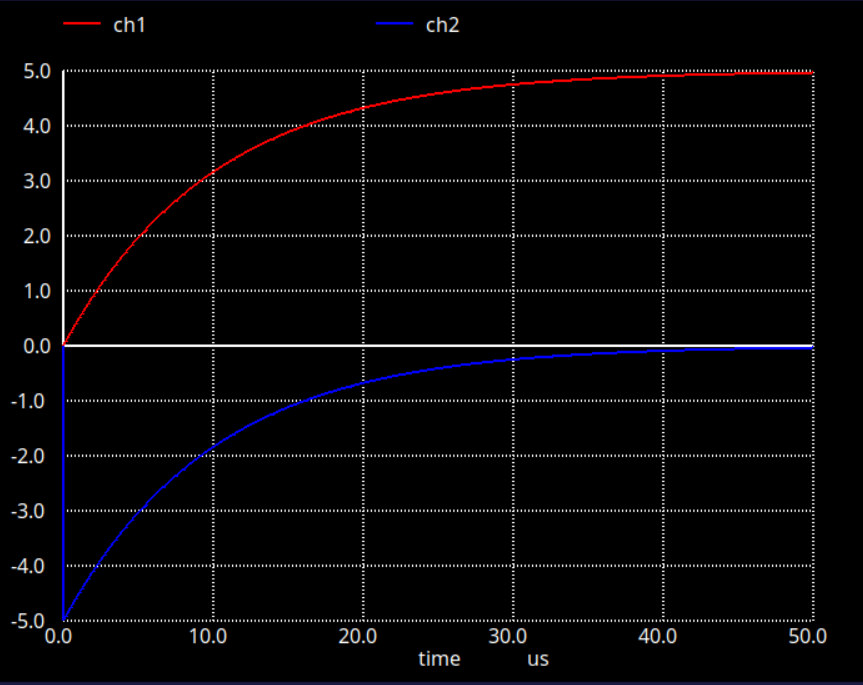
\includegraphics[width=0.75\linewidth]{Figs/plot_spice.png}
% \end{figure}
    
% \end{frame}


\end{document}
